\documentclass[a4paper,
fontsize=11pt,
%headings=small,
oneside,
numbers=noperiodatend,
parskip=half-,
bibliography=totoc,
final
]{scrartcl}

\usepackage{synttree}
\usepackage{graphicx}
\setkeys{Gin}{width=.8\textwidth} %default pics size

\graphicspath{{./plots/}}
\usepackage[ngerman]{babel}
\usepackage[T1]{fontenc}
%\usepackage{amsmath}
\usepackage[utf8x]{inputenc}
\usepackage [hyphens]{url}
\usepackage{booktabs} 
\usepackage[left=2.4cm,right=2.4cm,top=2.3cm,bottom=2cm,headheight=25.60228pt,includeheadfoot]{geometry}
\usepackage{eurosym}
\usepackage{multirow}
\usepackage[ngerman]{varioref}
\setcapindent{1em}
\renewcommand{\labelitemi}{--}
\usepackage{paralist}
\usepackage{pdfpages}
\usepackage{lscape}
\usepackage{float}
\usepackage{acronym}
\usepackage{eurosym}
\usepackage[babel]{csquotes}
\usepackage{longtable,lscape}
\usepackage{mathpazo}
\usepackage[flushmargin,ragged]{footmisc} % left align footnote

%%url brekas grrr
\def\UrlBreaks{\do\a\do\b\do\c\do\d\do\e\do\f\do\g\do\h\do\i\do\j\do\k\do\l%
\do\m\do\n\do\o\do\p\do\q\do\r\do\s\do\t\do\u\do\v\do\w\do\x\do\y\do\z\do\0%
\do\1\do\2\do\3\do\4\do\5\do\6\do\7\do\8\do\9\do\-}%

\usepackage{listings}

\urlstyle{same}  % don't use monospace font for urls

\usepackage[fleqn]{amsmath}

%adjust fontsize for part

%% geometry
\clubpenalty = 10000 
\widowpenalty = 10000 
\displaywidowpenalty = 10000
%% tightlist

\providecommand{\tightlist}{%
  \setlength{\itemsep}{0pt}\setlength{\parskip}{0pt}}

\usepackage{sectsty}
\partfont{\large}

%Das BibTeX-Zeichen mit \BibTeX setzen:
\def\symbol#1{\char #1\relax}
\def\bsl{{\tt\symbol{'134}}}
\def\BibTeX{{\rm B\kern-.05em{\sc i\kern-.025em b}\kern-.08em
    T\kern-.1667em\lower.7ex\hbox{E}\kern-.125emX}}

\usepackage{fancyhdr}
\fancyhf{}
\pagestyle{fancyplain}
\fancyhead[R]{\thepage}

%meta

%meta

\fancyhead[L]{A. Pohl \& F. Steeg \\ %author
LIBREAS. Library Ideas, 29 (2016). % journal, issue, volume.
\href{http://nbn-resolving.de/urn:nbn:de:kobv:11-100238146
}{urn:nbn:de:kobv:11-100238146}} % urn
\fancyhead[R]{\thepage} %page number
\fancyfoot[L] {\textit{Creative Commons BY 3.0}} %licence
\fancyfoot[R] {\textit{ISSN: 1860-7950}}

\title{\LARGE{Zurück ins Web. Die Entwicklung eines neuen Webauftritts für die Nord\-rhein-West\-fälische Bibliographie (NWBib)}} %title %title
\author{Adrian Pohl \& Fabian Steeg} %author

\setcounter{page}{}

\usepackage[colorlinks, linkcolor=black,citecolor=black, urlcolor=blue,
breaklinks= true]{hyperref}

\date{}
\begin{document}

\maketitle
\thispagestyle{fancyplain} 

%abstracts
\begin{abstract}
\small
Am Hochschulbibliothekszentrum des Landes Nord\-rhein-West\-falen (hbz) wird
seit Anfang 2014 nach Vorgaben und unter Begutachtung der Uni\-ver\-si\-täts-
und Landesbibliotheken in Düsseldorf, Münster und Bonn ein neuer
Webauftritt für die Landesbibliographie Nord\-rhein-West\-falens, die
Nord\-rhein-West\-fälische Bibliographie (NWBib) entwickelt. Die Entwicklung
basiert auf der Web- Schnittstelle des Linked-Open-Data-Dienst lobid und
wird vollständig mit Open- Source-Software entwickelt. Aus der
Perspektive des Entwicklungsteams am hbz beschreibt der Artikel Kontext
und Durchführung des Projekts. Der Beitrag skizziert die historische
Entwicklung der NWBib mit Fokus auf die Beziehung der Bibliographie zum
World Wide Web (WWW), erläutert die Voraussetzungen für die
Neuentwicklung sowie die Leitlinien des Entwicklungsprozesses, gibt
einen Überblick über die Nutzung des neuen Webauftritts und die zur
Umsetzung verwendete Technologie. Abgeschlossen wir der Artikel mit
Lessons-Learned und einem Ausblick auf weitere Entwicklungen.
\end{abstract}

%body
Dieser Artikel beschreibt die Entwicklung eines modernen Webauftritts
für die Nord\-rhein-West\-fälische Bibliographie (abgekürzt NWBib) im
Kontext der historischen Entwicklung dieser Landesbibliographie. Der
Auftritt findet sich unter:

\begin{center}
\url{https://nwbib.de}
\end{center}

Die Aufgaben einer Landesbibliographie bestimmt Syre (2006, S. 34) wie
folgt:

\begin{quote}
Aufgabe einer Regionalbibliographie ist es, die Literatur über eine
Region, ihre historischen und aktuellen Teilgebiete, ihre Naturräume und
ihre Orte sowie die mit der betreffenden Region verbundenen
Persönlichkeiten (verstorbenen wie lebenden) zu verzeichnen. Deckt sich
der geographische Berichtsraum einer Regionalbibliographie mit den
Grenzen eines Bundeslandes, spricht man von einer Landesbibliographie.
\end{quote}

Dies gilt so auch für die Nord\-rhein-West\-fälische Bibliographie. In der
Selbstdarstellung des neuen Webauftritts\footnote{\url{https://nwbib.de}}
heißt es:

\begin{quote}
Die Nord\-rhein-West\-fälische Bibliographie (NWBib) verzeichnet die
Literatur über das Land Nord\-rhein-West\-falen, seine Regionen, Orte und
Persönlichkeiten, Literatur aus allen Lebens- und Wissensbereichen in
Geschichte und Gegenwart.
\end{quote}

\begin{quote}
Die NWBib ist eine der umfangreichsten Regionalbibliographien
Deutschlands. Sie erschließt nicht nur Bücher und Zeitschriften, sondern
auch Aufsätze und andere Medien wie etwa Karten, DVDs, Hörbücher und
elektronische Publikationen.
\end{quote}

Mit Stand April 2016 verzeichnet die NWBib mehr als 370.000
Literaturnachweise, davon mehr als 60 Prozent Aufsätze aus Zeitschriften
oder Sammelbänden.

Der Aufbau des neuen NWBib-Webauftritt begann im Januar 2014. Zunächst
war die Beendigung der Testphase (Beta) vom Entwicklungsteam für Ende
2014 geplant. Der offizielle Launch-Termin wurde jedoch mehrmals nach
hinten verschoben. Im April 2016 haben die Leitungen der
Landesbibliotheken mitgeteilt, dass das Angebot nun beworben werden
könne. Eine öffentliche Vorstellung des neuen Auftritts wird Ende August
im Rahmen der Feierlichkeiten zu 70 Jahren NRW stattfinden.

Dieser Beitrag skizziert die historische Entwicklung der NWBib mit Fokus
auf die Beziehung der Bibliographie zum World Wide Web (WWW), beschreibt
die Voraussetzungen für die Neuentwicklung sowie die Leitlinien des
Entwicklungsprozesses, gibt einen Überblick über die Nutzung des neuen
Webauftritts und die zur Umsetzung verwendete Technologie und schließt
mit Lessons Learned und einem Ausblick auf weitere Entwicklungen. Da
beide Autoren Teil des Software-Entwicklungsteams am
Hochschulbibliothekszentrum des Landes Nord\-rhein-West\-falen (hbz) sind,
wird die Entwicklungsperspektive gegenüber der Perspektive der
NWBib-Redaktion hier im Vordergrund stehen.

\section*{Rechtliche Voraussetzungen und
Verantwortlichkeiten}\label{rechtliche-voraussetzungen-und-verantwortlichkeiten}

Die \enquote{entscheidende Grundlage für die Bearbeitung einer
Landesbibliographie} liefert die Wahrnehmung des Pflichtexemplarrechts
(Syré 2006, S. 36). Wie in anderen Bundesländern üblich, wird auch die
NWBib von jenen Bibliotheken erstellt, die für die Sammlung und
Archivierung von Pflichtstücken zuständig sind. Im Unterschied zu
anderen Bundesländern sind die Erstellung, die Entwicklung und der
Betrieb der Nord\-rhein-West\-fälischen Landesbibliographie sogar im
Pflichtexemplargesetz verankert. So heißt es im \emph{Gesetz zur
Regelung des Pflichtexemplarrechts in Nord\-rhein-West\-falen}, §2:

\begin{quote}
\begin{enumerate}
\def\labelenumi{(\arabic{enumi})}
\item
  Die Aufgabe der Sammlung der Pflichtexemplare nehmen die Uni\-ver\-si\-täts-
  und Landesbibliotheken Bonn, Düsseldorf und Münster gemeinsam wahr.
  {[}\ldots{}{]}
\item
  Die Bibliotheken erstellen gemeinsam die Nord\-rhein-West\-fälische
  Bibliographie. Diese verzeichnet und erschließt die Medienwerke mit
  inhaltlichem Bezug zu Nord\-rhein-West\-falen unabhängig davon, ob sie
  innerhalb oder außerhalb Nord\-rhein-West\-falens verlegt werden.
\item
  Das Hochschulbibliothekszentrum des Landes Nord\-rhein-West\-falen
  unterstützt die Pflichtexemplarsammlung der Uni\-ver\-si\-täts- und
  Landesbibliotheken sowie die Herausgabe der Nord\-rhein-West\-fälischen
  Bibliographie durch die Entwicklung und den Betrieb von technischen
  Infrastrukturleistungen.
\end{enumerate}
\end{quote}

Entsprechend sieht auch die tatsächliche Arbeitsteilung aus: Die
Redaktionsstellen an den Uni\-ver\-si\-täts- und Landesbibliotheken Münster
und Düsseldorf arbeiten an der Erstellung und Pflege der NWBib, wobei
sie von der ULB Bonn unterstützt werden, die sich auf die Erfassung von
Monographien beschränkt. Das Hochschulbibliothekszentrum fungiert als
technischer Dienstleister für Betrieb und Entwicklung der
Erfassungsumgebung und des Webauftritts.\footnote{Die
  \enquote{technische Organisation und Präsentation der
  Nord\-rhein-West\-fälischen Bibliographie} ist auch in der Satzung des
  Hochschulbibliothekszentrums explizit genannt, s.
  https://www.hbz-nrw.de/ueberuns/satzung/ (§2, Abs. 3 a, Punkt 7).}

Für den Aufbau des neuen NWBib-Webauftritts war am hbz dasselbe Team
verantwortlich, das auch den hbz-Linked-Data-Dienst lobid (Linking Open
Bibliographic Data) betreibt. Das lobid-Team besteht aus zwei
Entwicklern (Pascal Christoph mit Schwerpunkt auf Datentransformation
und Fabian Steeg mit Schwerpunkt auf Webentwicklung) und einem
wissenschaftlichen Bibliothekar (Adrian Pohl, verantwortlich für
Metadatenstandards, Projektmanagement und Kommunikation).

\section*{Historie der NWBib}\label{historie-der-nwbib}

Die NWBib ist eine der jüngeren Landesbibliographien Westdeutschlands.
Ihre direkten Vorläufer sind die Westfälische Bibliographie, die ab 1954
erstellt wurde und den Zeitraum ab 1945 abdeckt und die Lippische
Bibliographie, die ab 1957 erstellt wurde.\footnote{Für eine
  umfassendere Darstellung der NWBib-Vorläufer siehe Haller und Mühl
  (2006), 305ff. Die Landesbibliotheken haben die Vorläufer der NWBib
  digitalisiert. Unter
  \url{http://digital.ub.uni-duesseldorf.de/nav/classification/5975540}
  findet sich eine Liste von digitalisierten Bibliographien mit Bezug
  auf das Rheinland und unter
  \url{http://www.ulb.uni-muenster.de/landesbibliothek/recherche/westfaelische-bibliographien/}
  mit Bezug auf Westfalen.} Mit der Nord\-rhein-West\-fälischen
Bibliographie wurden diese Vorläufer fortgeführt und um die
bibliographische Verzeichnung von Literatur über das Rheinland ergänzt.
Der erste Band der NWBib (Berichtsjahr 1983) ist 1984 erschienen.

\paragraph{EDV-gestützte
Druckproduktion}\label{edv-gestuxfctzte-druckproduktion}

Wie Schmidt (1998) darstellt wurde von Anfang an auf eine EDV-gestützte
Produktion gesetzt, auch wenn die Bibliographie zunächst allein als
Druckfassung erschien. Dennoch war der Aufwand zur Erstellung einer
gedruckten Bibliographie ungleich größer im Vergleich zur heute gängigen
Pflege einer Datenbank. Für die ersten zehn Bände beschreibt Schmidt
(1998) das Verfahren wie folgt:

\begin{quote}
Die Titel wurden jahrgangsweise maschinenschriftlich auf Erfassungsbögen
von den beiden Redaktionsstellen an der UB Düsseldorf und der UB Münster
ans HBZ gesandt, dort von Datenerfassungskräften maschinenlesbar als
EDT-Dateien erfaßt, von einer weiteren Redakteurin korrekturgelesen und
schließlich mit dem GID-Programm verarbeitet. Das Endprodukt waren vier
Magnetbänder für die jeweils vier Teile einer Druckausgabe, fertig
kodiert mit Steuerzeichen für die Weiterverarbeitung auf einer
Lichtsetzmaschine. Diese Bänder wurden vom HBZ einem durch Ausschreibung
ermittelten Druckhaus übergeben, welches über eine bestimmte
Lichtsetzanlage verfügen mußte, um die Satzsteuerzeichen der
Magnetbänder richtig lesen zu können.
\end{quote}

Bei der Datenerfassung und -korrektur waren also drei Abteilungen
beteiligt, ehe die Daten für den Druck vorbereitet werden konnten.
Haller und Mühl (2006, S. 312) nennen drei erhebliche Nachteile dieses
Verfahrens: Erstens der doppelte Schreibaufwand bei der Erfassung über
Datenerfassungsbögen und der Übertragung in ein besser maschinenlesbares
Format, zweitens das aufwändige Korrekturverfahren bei der jährlichen
Druckaufbereitung und -- am schwerwiegendsten -- drittens das Fehlen
einer Datenbank, was eine Dublettenkontrolle und die kontrollierte
Verschlagwortung mittels der Schlagwortnormdatei (SWD) unmöglich machte.

\paragraph{Mit LaTeX ins Web}\label{mit-latex-ins-web}

Ab der Herstellung des elften Bandes der NWBib (Jahrgang 1993) hat sich
das Verfahren geändert. Der Hauptgrund für die Umstellung des
Druckverfahrens war der Anschluss der ULBs Düsseldorf und Münster an den
hbz-Verbund Anfang der 1990er Jahre, womit die NWBib als Sub-System der
hbz-Verbunddatenbank geführt wurde. Dies ermöglichte nicht nur das
Einsparen von Personalressourcen bei der Druckproduktion, sondern auch
die Präsentation der NWBib im WWW.

Die gedruckte Version wurde nun mit der Software \emph{LaTeX}
vorbereitet. Dafür wurde aus der für den hbz-Verbundkatalog genutzten
Datenbanksoftware \emph{BIS} ein mit TeX-Steuerzeichen versehener Export
des jeweiligen NWBib-Jahrgangs generiert (Schmidt 1998). Als
Nebenprodukt des neuen Verfahrens konnte auf Basis der LaTeX-Datei mit
wenig Aufwand eine HTML-Version der NWBib erstellt werden. Mit Hilfe
freier Software und nach Aufbringen einer Personenwoche konnte
NWBib-Jahrgang 1993 als erstes WWW-Angebot des hbz 1996 bereitgestellt
werden. In Schmidt (1998) heißt es -- unter Nutzung des Kürzels
\enquote{NWB} für die NWBib:

\begin{quote}
Um das Marketing dieses zusätzlichen Angebotes der Bibliographie auf dem
Internet brauchten wir uns {[}\ldots{}{]} nicht zu kümmern, das haben
die Gesetze des World Wide Web sozusagen über nacht {[}sic{]} erledigt.
Die NWB-Seiten wurden schon bald von den Suchmaschinen entdeckt,
eingelesen und indiziert. So kann ein Benutzer auch über eine Recherche
in einer Suchmaschine wie zum Beispiel Alta Vista als Treffer auf eine
NWB-Seite geführt werden und dort dann mit den Navigationswerkzeugen
weitersuchen.
\end{quote}

Zusätzlich zur HTML-Variante der Bibliographie wurde 1996 auch der
NWBib-Altbestand in die hbz-Verbunddatenbank eingespielt, so dass die
gesamte NWBib über den hbz-OPAC durchsucht werden konnte. Datenbanken
können aber nicht durch Suchmaschinen indexiert werden -- man bezeichnet
derartige Angebote als Teil des \enquote{Deep Web} --, weshalb allein
das HTML-Angebot die Auffindbarkeit der NWBib über Web-Suchmaschinen
ermöglichte.

Ende der 1990er Jahre wurde das hbz-Verbundsystem auf die Software
\emph{Aleph} von Ex Libris umgestellt. Die NWBib-Redaktion nutzte diese
Chance, um die NWBib vollständig in den Verbundkatalog zu integrieren
(Haller und Mühl 2006, S. 314f), was unter anderem den Vorteil hatte,
dass die Nutzer jetzt auch Besitznachweise für die verzeichneten Titel
vorfanden. Laut Haller und Mühl (2006, S. 314) fiel mit \enquote{dem
Beschluss für eine vollständige Übernahme der Bibliographie in das neue
Verbundsystem {[}\ldots{}{]} auch die Entscheidung, die Druckausgabe
aufzugeben und die Bibliographie nur noch als Datenbank anzubieten.} Die
letzte Druckausgabe der NWBib erschien 1999 mit Berichtsjahr 1997.

2005 wurde auch die HTML-Version der NWBib eingestellt, und es gab nur
noch die Möglichkeit einer Recherche über den Web-OPAC, der mittlerweile
auf dem Aleph-System von von Ex Libris basierte. Damit verschwand die
NWBib aus dem WWW, und die verzeichnete Literatur war nur für die Leute
recherchierbar, die von der Existenz der Bibliographie und ihren
Möglichkeiten wussten.

\paragraph{Der Auftrag zur Modernisierung des
Web-Auftritts}\label{der-auftrag-zur-modernisierung-des-web-auftritts}

Mit dem Aufstieg von Google und Dis\-covery-Services in den Bibliotheken
wurde die NWBib-Recherche immer weniger zeitgemäß. Als Reaktion gaben
die Landesbibliotheken dem hbz Anfang 2013 den Auftrag, den Webauftritt
der NWBib zu überarbeiten. Innerhalb des hbz wurde entschieden, den
neuen Webauftritt auf Basis der Programmierschnittstelle (Application
Programming Interface, API) des hbz-Linked-Data-Dienstes lobid
umzusetzen, die im Herbst 2013 in Produktion gegangen war. Dies sollte
unter anderem garantieren, dass die NWBib -- wie bereits knapp zwanzig
Jahre zuvor -- wieder integraler Bestandteil des WWW würde. Anfang 2014
begannen die Entwicklungsarbeiten für den neuen NWBib-Webauftritt.

\section*{Anforderungen an einen modernen
Webauftritt}\label{anforderungen-an-einen-modernen-webauftritt}

Welche Anforderungen sollte ein moderner Webauftritt erfüllen? Schnasse
(2015) hat für einen NWBib-Vortrag beim Bibliothekartag 2015 in Nürnberg
eine nützliche Untergliederung von Interessengruppen eines
bibliographischen Webauftritts und deren Anforderungen erstellt, an der
wir uns hier orientieren.\footnote{Siehe Schnasse (2015), Folie 5.} Es
lassen sich vier Interessengruppen unterscheiden:

\begin{enumerate}
\def\labelenumi{\arabic{enumi}.}
\tightlist
\item
  Besucher der NWBib, die nach Literatur recherchieren,
\item
  Externe Webservices, zum Beispiel Suchmaschinen wie Google, DuckDuckGo
  oder die Virtuelle Deutsche Landesbibliographie (VDL),
\item
  die NWBib-Redaktion sowie
\item
  Web-Entwickler, die auf Basis der NWBib-Daten zusätzliche eigene
  Anwendungen bauen wollen.
\end{enumerate}

Im Folgenden werden die Anforderungen der verschiedenen Nutzergruppen
näher beleuchtet.

\paragraph{NWBib-Besucher}\label{nwbib-besucher}

Das Ziel von Nutzerinnen und Nutzern einer bibliographischen
Rechercheanwendung ist es, Literaturhinweise zu einem bestimmten Thema
sowie Hinweise zu Zugriffsmöglichkeiten zu bekommen, im besten Fall mit
einem direkten Link zum Volltext. Darüber hinaus erwarten Nutzerinnen
und Nutzer im Allgemeinen von einer Webanwendung folgende grundlegende
Eigenschaften:

\begin{itemize}
\tightlist
\item
  Verlässlichkeit/Verfügbarkeit
\item
  Übersichtlichkeit
\item
  Intuitive Nutzbarkeit
\item
  Schnelle Ladezeiten
\end{itemize}

Über diese allgemeinen Anforderungen hinaus variieren die Anforderungen
je nach Nutzungstypus. Eine regelmäßig wiederkehrende Besucherin, die
etwa spezielle wissenschaftliche Literatur sucht, wird andere Wünsche
und Anforderungen haben als ein Besucher, der über eine Google-Suche
direkt auf einen Einzeltreffer gelangt. Letzterer will sich erst einmal
auf einfache Weise orientieren, auf was für eine Seite er da gelangt ist
und welche Informationen sie ihm bietet. Letztere könnte hingegen
Interesse haben, komplexere Recherchefunktionen einzusetzen.

Bisher wurde darauf verzichtet, systematisch herauszufinden, wie
zufrieden Endnutzerinnen und Endnutzer mit dem NWBib-Webauftritt sind
und welche Dinge verbesserungswürdig sind. Im Zuge der kontinuierlichen
Weiterentwicklung des Auftritts sind Usability-Studien für das Jahr 2017
geplant.

\paragraph{Externe Webservices}\label{externe-webservices}

Externe Websites lassen sich in verschiedene Typen mit unterschiedlichen
Anforderungen an eine Rechercheanwendung untergliedern:

\begin{itemize}
\tightlist
\item
  \emph{Suchmaschinen} crawlen große Mengen von Webseiten und verwerten
  zunehmend darin angebotene strukturierte Daten.
\item
  Andere möchten die NWBib über eine dokumentierte Schnittstelle
  abfragen und strukturierte Daten als Antwort bekommen, um die
  Ergebnisse in ihrem Webauftritt präsentieren. Dazu zählt zum Beispiel
  die Virtuelle Deutsche Landesbibliographie (VDL).
\item
  Andere wie die \emph{Website der NRW-Landesbibliotheken}\footnote{Siehe
    \url{http://www.landesbibliothek-nrw.de/}.} möchten die
  NWBib-Anwendung als Ganzes -- inklusive erweiterter Suchmaske und
  Facettierungsmöglichkeiten -- in ihren Webauftritt integrieren.
\end{itemize}

\paragraph{NWBib-Redaktion}\label{nwbib-redaktion}

Die NWBib-Redaktion bewertet die Funktionalitäten des NWBib-Auftritts in
erster Linie vor dem Hintergrund der von ihr erfassten Daten, dem dabei
benutzten Regelwerk zur Formalerschließung und den verschiedenen
Methoden zur Inhaltserschließung.

Konkret erwartet die NWBib-Redaktion zum Beispiel folgende
Funktionalität:

\begin{itemize}
\tightlist
\item
  Angeboten werden sollte eine erweiterte Suche über verschiedene
  Felder, die mittels Boolescher Operatoren kombiniert werden können.
\item
  Die Ergebnismenge einer Anfrage soll mit jener in der Aleph-Recherche
  übereinstimmen, was etwa Methoden wie Stemming oder ähnliches
  ausschließt.
\item
  Die Ergebnisliste soll standardmäßig nach Erscheinungsjahr sortiert
  sein.
\item
  Treffer sollten auf eine Merkliste gesetzt werden können, die
  exportiert werden kann.
\end{itemize}

So hat die Redaktion zum Ziel, dass die Daten entsprechend den Feldern,
Unterscheidungen, Verknüpfungen und Details in den Ausgangsdaten
präsentiert werden. Die -- teils komplexen -- Recherchemöglichkeiten,
die die Datenbasis ermöglicht, sollen ausgenutzt werden.

Die NWBib-Redaktion ist jener Stakeholder, der bisher am meisten
Einfluss auf den Entwicklungsprozess nehmen konnte.

\paragraph{Web-Entwickler}\label{web-entwickler}

Grundsätzlich versucht das hbz mittels dem lobid-Dienst, offene
bibliothekarische Daten so bereitzustellen, dass interessierte Dritte
diese innerhalb eigener Anwendungen nutzen können. Damit Entwickler die
Daten in eigenen Webanwendungen integrieren können, benötigen sie gut
dokumentierte, performante und zuverlässige Schnittstellen zu den Daten.
Zudem sollten die angebotenen Daten bestenfalls explizit offen
lizenziert sein.

\section*{Bibliothekarische
Voraussetzungen}\label{bibliothekarische-voraussetzungen}

Wie bereits erwähnt wird die NWBib als Untermenge des
hbz-Verbundkatalogs mit der Software \emph{Aleph} der Firma Ex Libris
katalogisiert. Zur Identifizierung von NWBib-Titeln wird ein Kennzeichen
in Feld 078n gesetzt.\footnote{Dem lobid-Dienst liegt ein Export aus dem
  Verbundsystem im Format \enquote{Aleph-Sequentials} zugrunde. Ein
  Beispiel NWBib-Titel in diesem Format findet sich unter
  \url{http://lobid.org/hbz01/HT018881872}.}

Die Titelerfassung für die NWBib geschieht nach den \emph{Regeln für die
alphabetische Katalogisierung in wissenschaftlichen Bibliotheken}
(RAK-WB) und seit Beginn dieses Jahres nach \emph{Resource Description
and Access} (RDA). Die Inhaltserschließung wird zum einen nach den
\emph{Regeln für den Schlagwortkatalog} (RSWK) mithilfe der Gemeinsamen
Normdatei (GND) durchgeführt und insbesondere die ULB Münster arbeitet
an der Verzeichnung von Schlagwortfolgen, die auch im neuen Webauftritt
nutzbar gemacht werden. Zum anderen erfolgt eine Klassifizierung anhand
einer NWBib-spezifischen Systematik, die in einen Sachsystematik- und
einen Raumsystematikteil\footnote{Siehe
  \url{http://nwbib.de/classification?t=Sachsystematik} und
  \url{http://nwbib.de/classification?t=Raumsystematik}.} untergliedert
ist. Ergänzt wird die NWBib-Raumsystematik zudem durch sogenannte
\enquote{Gliedernde Schlagwörter}, das sind unkontrollierte Einträge von
Ortsnamen zur genaueren räumlichen Verortung des Sachbezugs eines
Titels.

\section*{Der Webauftritt}\label{der-webauftritt}

Die Startseite des neuen NWBib-Webauftritts bietet ein Suchfeld für den
einfachen Einstieg, eine Beschreibung der NWBib sowie eine Karte für die
Eingrenzung nach Ortsbezug, bei der zwischen Kreis- oder Gemeindeebene
gewählt werden kann:

\begin{figure}[htbp]
\centering
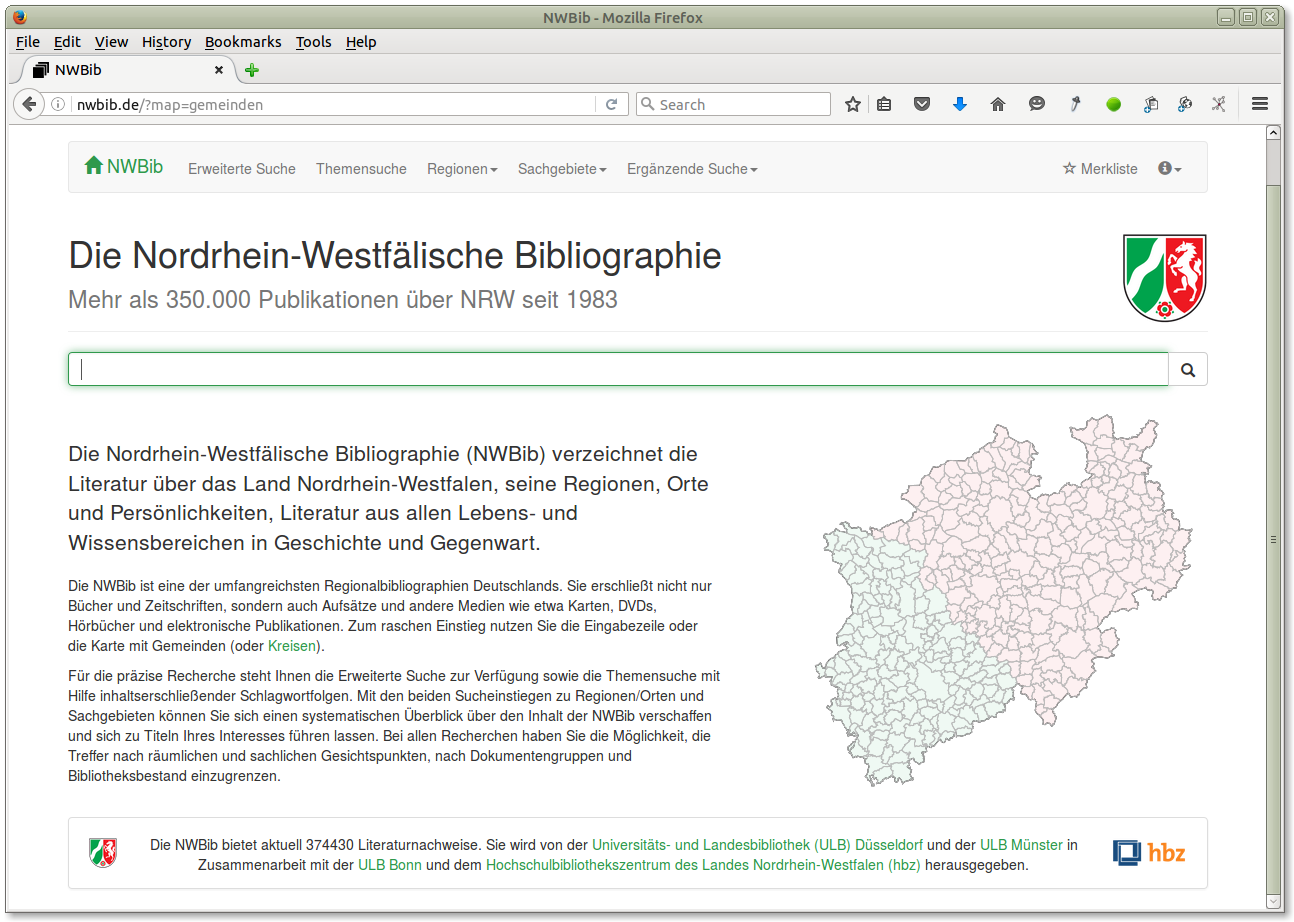
\includegraphics{img/nwbib-screenshot-startseite.png}
\caption{Startseite}
\end{figure}

Über das Suchfeld und die kartenbasierte Ortsfacette -- an der rechten
Seite unter \enquote{Ortsbezug} -- können auf einfache Weise inhaltliche
und räumliche Suchkriterien kombiniert werden oder nach
Erscheinungsjahr(en) gefiltert werden. Hier zum Beispiel wurde die
textbasierte Suche nach \enquote{braunkohle} durch eine Auswahl in der
Karte auf eine Suche von Literatur über Braunkohle im rheinischen
Braunkohlerevier eingeschränkt:

\begin{figure}[htbp]
\centering
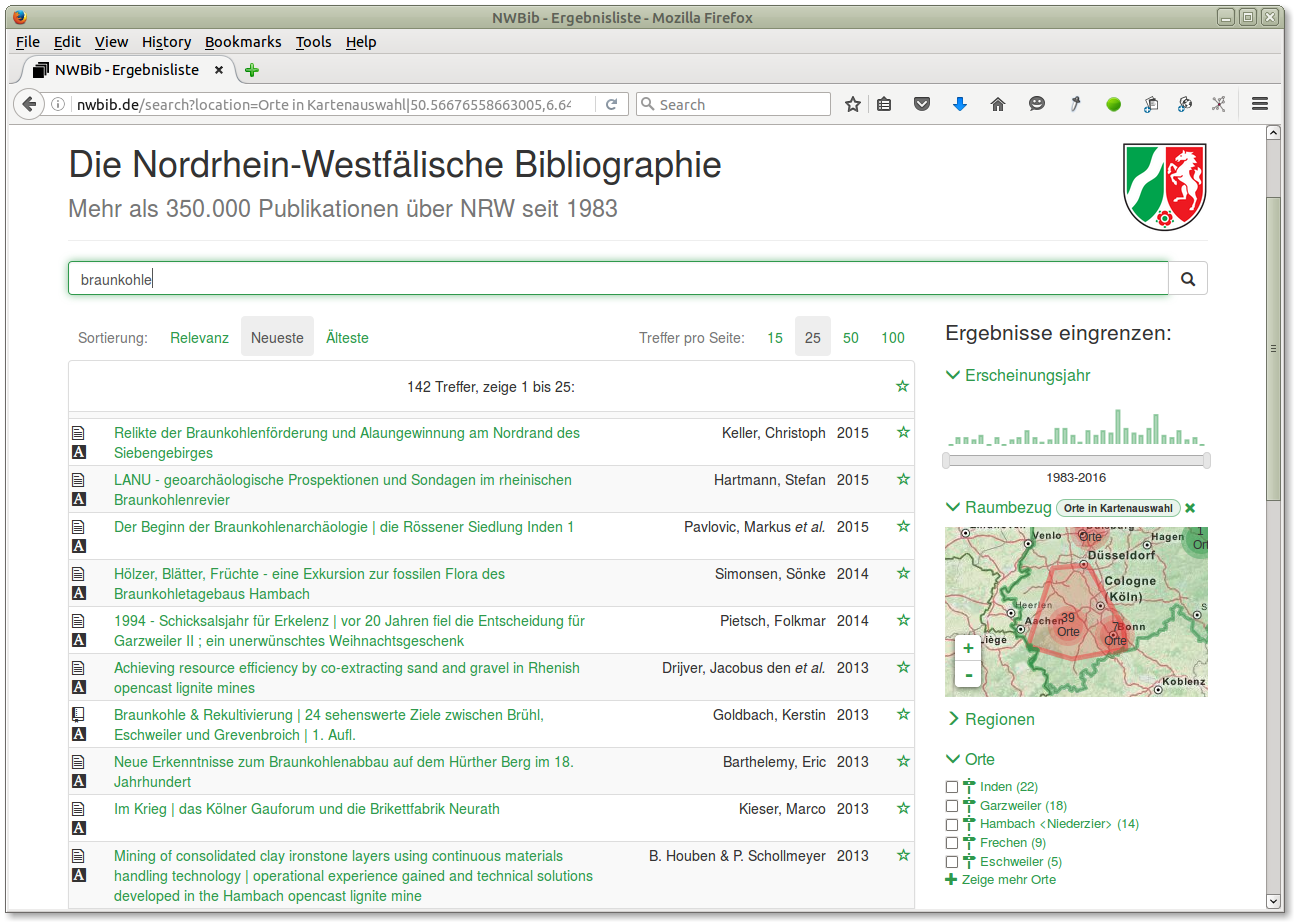
\includegraphics{img/nwbib-screenshot-ergebnisliste.png}
\caption{Ergebnisliste}
\end{figure}

Weitere Facetten rechts neben der Suchergebnisliste bieten Möglichkeiten
zur Einschränkung der Ergebnisse nach inhaltlichen Kriterien, nach
Medien- und Publikationstypen, sowie nach Bestand in bestimmten
Bibliotheken:

\begin{figure}[htbp]
\centering
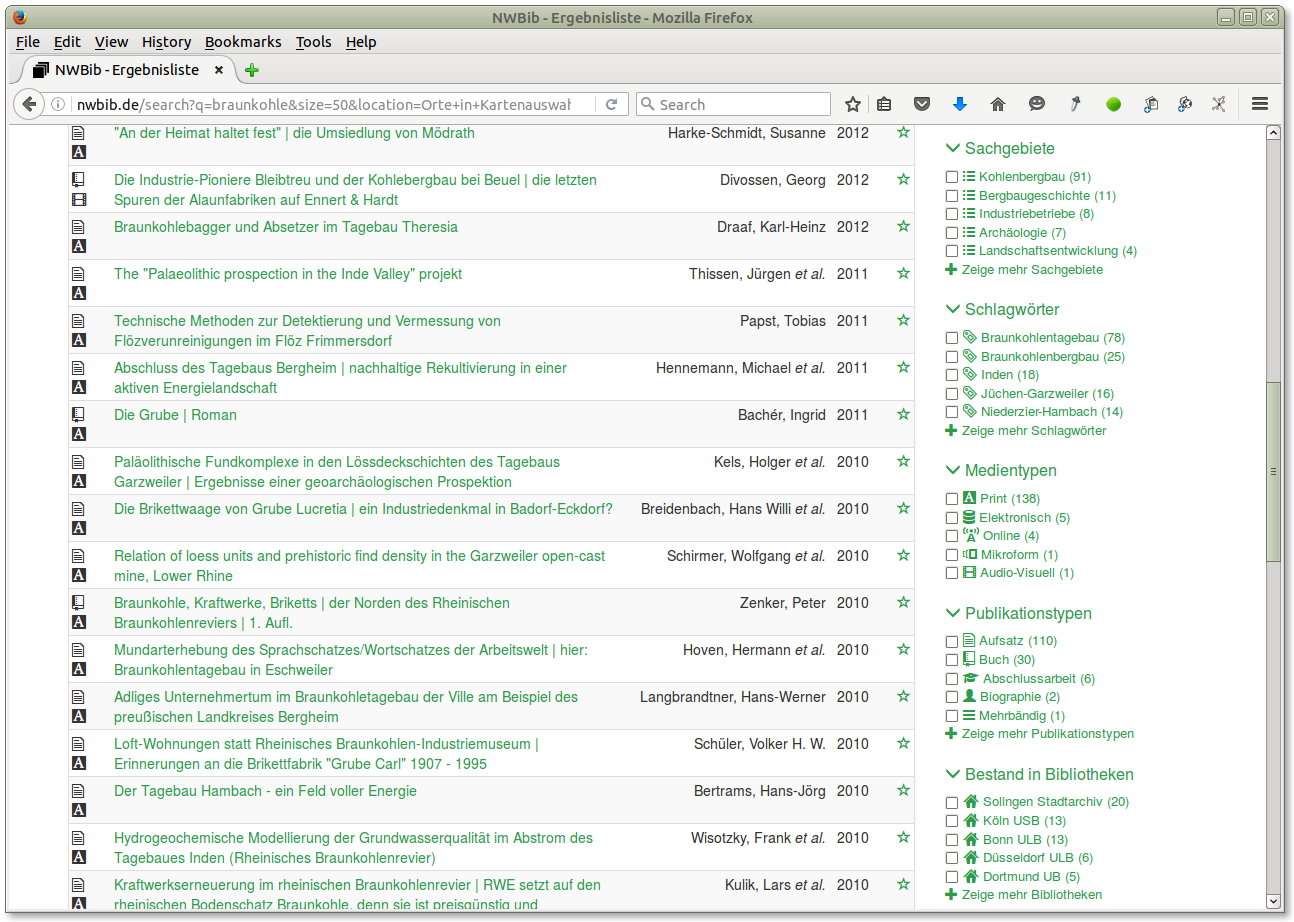
\includegraphics{img/nwbib-screenshot-facetten.png}
\caption{Facetten}
\end{figure}

Die Detailansicht eines Treffers bietet über Links Möglichkeiten zum
Suchen nach weiteren Treffern desselben Urhebers und derselben
inhaltlichen Erschließung sowie auf einer Karte Details zum Bestand und,
wenn verfügbar, Links zum Abfragen der Verfügbarkeit im lokalen Katalog
der Bibliotheken:

\begin{figure}[htbp]
\centering
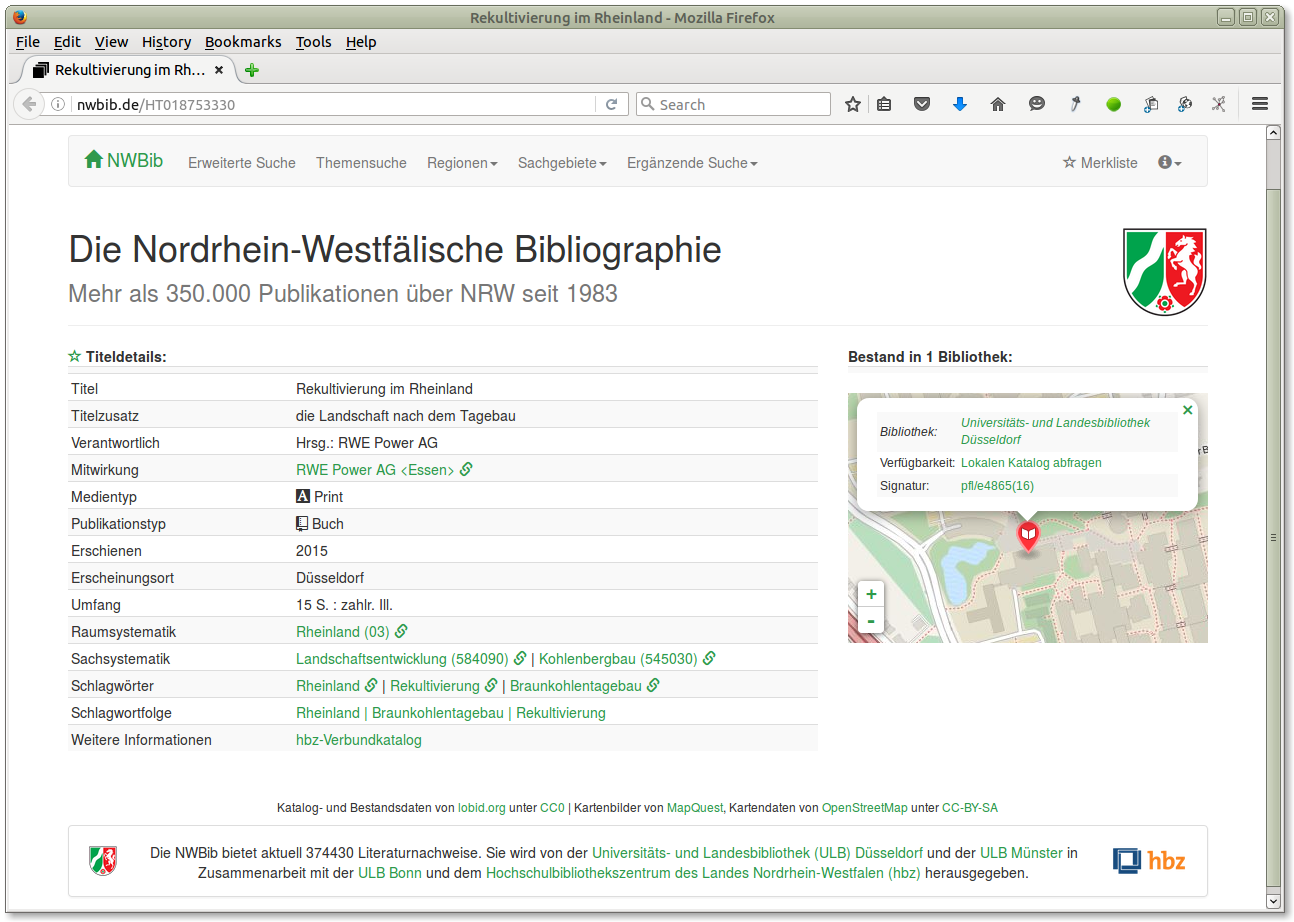
\includegraphics{img/nwbib-screenshot-detailansicht.png}
\caption{Detailansicht}
\end{figure}

Neben dieser grundsätzlichen Funktionalität bietet der Auftritt über die
Menüleiste eine erweiterte Suche in bestimmten Feldern, eine Themensuche
über inhaltserschließende Schlagwortfolgen, Zugriff auf Titel über die
Raum- und Sachsystematik, sowie mit der Merklistenfunktion die
Möglichkeit zum Zusammenstellen und Drucken einer Literaturliste.

\section*{Der Entwicklungsprozess}\label{der-entwicklungsprozess}

Die Software für den neuen NWBib-Webauftritt wird schrittweise in
stetigem Austausch mit der NWBib-Redaktion entwickelt. Der
Entwicklungsprototyp ist seit Beginn der Entwicklung offen im Web
erreichbar und dient als Referenzpunkt für die Diskussion über offene
Anforderungen und bestehende Softwarebugs. An ihm wird kontinuierlich
weiterentwickelt (inkrementelle Entwicklung). Für verschiedene
Recherchefunktionen sowie teilweise auch für die Einzeltrefferanzeige
konnte zudem die Aleph-basierte Version der NWBib als Referenz
herangezogen werden.

\paragraph{Rollen und Kommunikation}\label{rollen-und-kommunikation}

Für die technische Entwicklung des NWBib-Webauftritts setzt das
Entwicklungsteam im hbz die Anforderungen der NWBib-Redaktion um. Für
die Kommunikation zwischen dem Entwicklungsteam und der NWBib-Redaktion
ist der wissenschaftliche Bibliothekar verantwortlich, der auch die
Rolle des Product-Owners innehat. Die drei Mitglieder des
Entwicklungsteams arbeiten im Projektverlauf zusammengenommen etwa im
Umfang von einer Vollzeitstelle an dem Projekt.

Um die Anforderungen zu definieren, zu priorisieren, umzusetzen und die
erfolgreiche Umsetzung abzunehmen, müssen die beteiligten Akteure viel
und regelmäßig miteinander kommunizieren. Dies geschah in erster Linie
über eine gemeinsame Mailingliste und ein Wiki\footnote{Siehe
  \url{https://wiki1.hbz-nrw.de/x/mYyW}.}. Zudem gab es im September
2014 und April 2015 zwei persönliche Treffen im hbz.

Zunächst dienten verschiedene von der Redaktion verschickte oder beim
gemeinsamen Treffen erstellte Anforderungslisten als
Entwicklungsvorgaben. Da Fragen der Priorisierung teilweise unklar waren
und das Entwicklungsteam einen baldigen Launch des neuen Webauftritts
anvisierte, wurden nach etwa einem Jahr Entwicklung im Februar 2015 die
verbliebenen Anforderungen durch die NWBib-Redaktion zusammengeführt und
priorisiert. So entstand eine strukturierte Übersicht von Anforderungen,
die für den Launch des neuen NWBib-Webauftritts als unverzichtbar
angesehen werden.\footnote{Siehe
  \url{https://wiki1.hbz-nrw.de/x/CoCDAw}.} Diese Liste wird seitdem
regelmäßig an den Stand der Entwicklung angepasst und dient als
Bezugspunkt für die Entwicklung und die Kommunikation zwischen den
Projektbeteiligten. Mit der Zeit mussten einige der Anforderungen
konkretisiert beziehungsweise in detailliertere Aufgabenpakete
aufgeteilt werden.

Der typische Ablauf zur Umsetzung von Anforderungen sah wie folgt aus:

\begin{enumerate}
\def\labelenumi{\arabic{enumi}.}
\tightlist
\item
  Eine Anforderung oder ein Software-Bug wird von der Redaktion
  gemeldet.
\item
  Der Product-Owner legt ein oder mehrere Tickets für die Umsetzung der
  Anforderung beziehungsweise die Behebung des Bugs an.
\item
  Der Product-Owner priorisiert die offenen Tickets gemeinsam mit dem
  Rest des Entwicklungsteams und weist das Ticket einem Entwickler zu.
\item
  Der Entwickler arbeitet so lange an der Umsetzung des Tickets, bis er
  meint, dass die Anforderungen erfüllt werden.
\item
  Die neue beziehungsweise reparierte Funktionalität und der Code wird
  durch Mitglieder des Entwicklungsteams begutachtet.
\item
  Sobald die Begutachtung positiv ist, wird die Anpassung auf dem offen
  einsehbaren Entwicklungsprototyp produktiv.
\item
  Ist eine relevante Anzahl von Änderungen produktiv (dies sind meist
  fünf oder mehr Anpassungen), schickt der Product-Owner eine Mail an
  die gemeinsame NWBib-Mailingliste mit der Bitte um Begutachtung durch
  die NWBib-Redaktion.
\item
  Die NWBib-Redaktionsstellen stimmen sich untereinander ab, ob die
  Anpassungen den Anforderungen genügen. Sodann melden sie das Ergebnis
  der Abstimmung via Mailingliste an das Entwicklungsteam.
\item
  Ist die Rückmeldung positiv, wird die Entwicklung der Funktionalität
  als abgeschlossen erklärt, indem die Anforderung im Wiki entsprechend
  markiert wird. Andernfalls arbeitet das Entwicklungsteam an der
  gewünschten Anpassung und der Prozess setzt wieder bei Punkt 4. ein.
\end{enumerate}

Das Entwicklungsteam arbeitete nicht ausschließlich an der NWBib und die
Abstimmung der NWBib-Redaktionsstellen zur Begutachtung des Fortschritts
nahm einige Zeit in Anspruch. Die Länge eines Entwicklungszyklus vom
Melden einer Anforderung/eines Bugs bis zur endgültigen Abnahme durch
die Redaktion variierte in Abhängigkeit der Anwesenheit der Beteiligten
erheblich: Wenn keine Urlaubszeit war und alle Beteiligten da waren,
dauerte ein Zyklus zwei bis drei Wochen, in Abwesenheit des
Hauptentwicklers mehrere Monate.

Neben den Anforderungen der NWBib-Redaktion hat das Entwicklungsteam
auch eigene Vorstellungen umgesetzt. So wurden manche Anwendungsfälle
durch andere Funktionalitäten gelöst als ursprünglich von der Redaktion
gefordert. In anderen Fällen setzte das Entwicklungsteam eigene Ideen um
-- so etwa der kartenbasierte Sucheinstieg und die Visualisierung von
Suchergebnissen und Bestandsinformationen auf einer Karte. Auch diese
Umsetzungen wurden dann der Redaktion zur Begutachtung vorgelegt
(Schritt 7) und durch deren Rückmeldungen entscheidend verbessert.

\paragraph{Entwicklungsmethode}\label{entwicklungsmethode}

Die Entwicklung des NWBib-Auftritts bedient sich bei verschiedenen
Ansätzen der agilen Softwareentwicklung (Beck 2001).\footnote{Für eine
  detaillierte Beschreibung des Entwicklungsprozesses im lobid-Team
  (allerdings in Englisch) siehe http://hbz.github.io/\#dev-process.
  \url{https://hbz.github.io/\#dev-process}.} Die Software wird -- wie
bereits beschrieben -- inkrementell in stetigem Austausch mit der
NWBib-Redaktion entwickelt. Als Kommunikationswerkzeuge benutzt das
Entwicklungsteam vor allem GitHub sowie zusätzlich zur Visualisierung,
Priorisierung und Organisation der Aufgaben die GitHub-basierte
Kanban-Soft\-ware \emph{Waffle}.\footnote{Siehe das gemeinsame
  Waffle-Board für alle Projekte des lobid-Teams:
  https://waffle.io/hbz/lobid} Vom Scrum-Ansatz (Pichler 2009) wird das
Stand-up übernommen, ein kurzes tägliches Treffen, bei dem sich die
Teammitglieder über ihre erledigten und anstehenden Aufgaben austauschen
und aktuelle Probleme benennen. Der Entwicklungsprozess folgt dem
GitHub-Flow.\footnote{Siehe
  \url{https://guides.github.com/introduction/flow/} sowie die
  Dokumentation des lobid-Entwicklungsprozesses:
  \url{http://hbz.github.io/\#dev-process}.}

\section*{Technologie}\label{technologie}

Die Implementierung des NWBib-Webauftritts verwendet Java- und
Web-Technologie und basiert komplett auf Open-Source-Software.\footnote{Software
  und Infrastruktur finden sich unter \url{http://github.com/hbz/nwbib}}

\paragraph{Überblick}\label{uxfcberblick}

Wie oben beschrieben, werden die Daten der NWBib im Bibliothekssystem
Aleph katalogisiert. Die Daten werden in einem XML-Format exportiert und
mithilfe des Datentransformationstools \emph{Metafacture} in JSON-LD
(JavaScript Object Notation - Linked Data) umgewandelt. Diese JSON-Daten
werden in Elastic\-search indexiert und über die Lobid-API im Web
bereitgestellt. Die NWBib-Webanwendung greift über HTTP auf diese API
zu. API und NWBib sind auf Basis des Play-Frameworks implementiert, die
NWBib verwendet zusätzlich das HTML-CSS-Framework Bootstrap.

Die folgende Abbildung bietet einen Überblick über diese Komponenten und
den Datenfluss aus Aleph in die NWBib:

\begin{figure}[htbp]
\centering
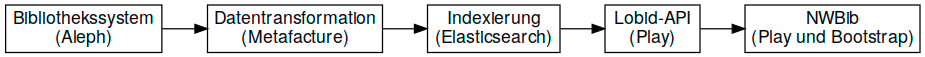
\includegraphics{img/data-workflow.png}
\caption{Datenfluss}
\end{figure}

Java-basierte Ansätze zur Entwicklung von Webanwendungen sind im
Bibliothekswesen nach unserem Eindruck relativ selten. Wir wollen daher
an dieser Stelle einen kurzen Einblick in die von uns verwendete
Technologie und den damit verbundenen Ablauf der Webentwicklung geben.
Auf die nur indirekt über die Lobid-API verwendeten Komponenten
Metafacture und Elasticsearch gehen wir an dieser Stelle nicht ein.

\paragraph{Webentwicklung mit Java}\label{webentwicklung-mit-java}

Historisch betrachtet hat Webentwicklung mit Java den Ruf,
schwergewichtig und komplex zu sein. Dies liegt vor allem an den
Frameworks und Tools, die als Teil der Java-Enterprise-Edition (Java-EE,
früher J2EE) zum Einsatz kommen. Applikationsserver und GUI-Frameworks
(zum Beispiel Java-Server-Faces, JSF), die als Abstraktionsschicht das
Hypertext-Transfer-Protocol (HTTP) vom Entwickler wegkapseln, sind unter
bestimmten Umständen für die Entwicklung von Unternehmenssoftware in
großen Teams geeignet, für typische Webapplikationen aber häufig nicht
optimal.

Hier haben sich leichtgewichtigere Frameworks und Technologien wie PHP
und Ruby on Rails etabliert. Diese sind näher an den zugrundeliegenden
Web-Technologien wie HTTP und HTML und erlauben einen schnelleren
Entwicklungszyklus: Änderungen im Quellcode werden einfach gespeichert
und die Seite im Browser neu geladen. Diese Vorteile dynamischer
Sprachen wie PHP, Perl oder Ruby überwiegen gerade in Projekten mit nur
einem Entwickler deren Nachteile, speziell die höhere Fehleranfälligkeit
durch dynamische Typisierung.

Eine statische Typisierung wie in Java hat neben einer höheren
Laufzeitperformanz auch für die Arbeit im Team Vorteile: Viele Fehler,
die durch Änderungen im Quellcode eingeführt werden, werden durch die
Typisierung früh erkannt, nämlich nicht erst bei der Verwendung einer
bestimmten Funktionalität, zum Beispiel beim Zugriff auf eine bestimmte
Seite, sondern schon bei der Kompilierung des Quellcodes, und damit
bevor die Seite überhaupt aufgerufen wird. Die Überprüfung kann zudem
sehr einfach automatisiert werden, so dass der fehlerhafte Code erst gar
nicht ins Code-Repository hochgeladen wird.

\paragraph{Webentwicklung mit Play}\label{webentwicklung-mit-play}

Das von uns verwendete Play-Framework verbindet die Vorteile der
schnellen Entwicklungszyklen und Web-nativen Entwicklung mit der
Typsicherheit von Java: Bei der Verwendung des Play-Frameworks können
wie bei PHP oder Rails nach dem Editieren des Quellcodes die Seiten
einfach neu geladen werden. Die nötige Kompilierung erfolgt inkrementell
und on-the-fly im Hintergrund.

Wesentliche Komponenten bei der Webentwicklung mit Play sind Routen,
Controller und Templates:

\begin{itemize}
\tightlist
\item
  \emph{Routen} beschreiben die HTTP-URLs der Anwendung, deren
  Query-Parameter und den entsprechenden Controller-Aufruf.
\item
  \emph{Controller} werden bei Aufruf der entsprechenden URLs
  ausgeführt. Sie verarbeiten den ankommenden HTTP-Request und erzeugen
  eine HTTP-Response, zum Beispiel mit dem Ergebnis eines
  Template-Aufrufs.
\item
  \emph{Templates} erzeugen das darzustellende HTML und können dazu
  beliebige aus den Controllern übergebene Daten verwenden.
\end{itemize}

Alle drei Komponenten werden dabei von Play typsicher verarbeitet. Wird
etwa eine Route definiert, bei der zum Beispiel ein \texttt{size}
Parameter vom Typ \texttt{Int} an einen Controller übergeben wird, der
einen \texttt{String} erwartet, erkennt der Compiler dies beim Start der
Anwendung. Ebenso wenn etwa im Template ein Wert als \texttt{String}
verwendet wird, der aber im Controller als \texttt{JsonNode} übergeben
wurde. Fehler in Routen, Controllern und Templates werden somit früh
erkannt, ohne dass dazu erst die betroffene Funktionalität der Anwendung
ausgeführt werden muss.

So ermöglicht das Play-Framework moderne Web-Entwicklung nah am HTTP,
mit effizienten Entwicklungszyklen, performanter Laufzeit und
typsicherem Code.

\section*{Herausforderungen \& Lessons
Learned}\label{herausforderungen-lessons-learned}

Im Laufe des Projekts sind den Beteiligten einige Herausforderungen
begegnet, und das lobid-Team hat eine Menge gelernt. Im folgenden werden
einige Herausforderungen und Lessons Learned aus Sicht des
Entwicklungsteams erläutert.

\paragraph{Daten und Recherche}\label{daten-und-recherche}

Wie oben beschrieben basiert die NWBib auf der lobid-API, die unter
anderem Zugriff auf die hbz-Verbundkatalogdaten sowie die Daten des
deutschen ISIL-Verzeichnisses ermöglicht. Für die Bereitstellung der
lobid-API werden die Quelldaten, die in einem Aleph-XML-Exportformat
(hbz-Verbunddaten) sowie Pica+-XML (ISIL-Daten) vorliegen, nach JSON-LD
überführt. Die Transformation von bibliothekarischen MAB-/MARC-basierten
Daten in eine für Entwickler leicht zu nutzende Datenstruktur ist nicht
trivial. Auch wenn für die Bereitstellung der lobid-API bereits eine
Menge Vorarbeiten stattgefunden hatten, mussten im Zuge der Entwicklung
des neuen NWBib-Webauftritts einige Herausforderungen auf Datenebene
gemeistert werden, um die gewünschten Funktionalitäten anbieten zu
können.

\emph{JSON-LD und Elasticsearch}: Ein grundlegendes Problem mit dem
JSON-LD, das in die Elasticsearch-Suchmaschine indexiert wird, war schon
seit Anfang 2014 bekannt. Die verwendeten existierenden
Java-JSON-LD-Tools bieten beschränkte Möglichkeiten zur Überführung von
N-Triples in JSON-LD, so dass das resultierende JSON-LD nicht die
optimale Struktur aufweist. Es hat keine geschachtelte Baumstruktur,
sondern ein flache Struktur, so dass sich viele Möglichkeiten der
Suchmaschine nicht nutzen lassen. Als Ergebnis wurde im Mai 2014 die
Planung für eine Version 2.0 der lobid-API begonnen. Die Generierung
eines für Elasticsearch optimierten JSON-LD ist eines der Hauptziele.
Die lobid-API 2.0 soll bis zum Herbst dieses Jahres produktiv gehen.

\emph{Körperschaftssuche}: Die NWBib-Redaktion verlangt eine
Suchmöglichkeit bibliographischer Ressourcen auf Basis von beteiligten
Körperschaften. Da bei der bisherigen Datenmodellierung ein solcher
Anwendungsfall nicht berücksichtigt wurde, waren einige temporäre
Anpassungen nötig, um eine Körperschaftssuche anbieten zu können. Für
die erwähnte komplette Neuüberarbeitung der Datenstrukturen (lobid-API
2.0) wurde schließlich beschlossen, analog zu den Quelldaten eine
grundlegende Unterscheidung von Körperschaften und Personen auf
Feldebene umzusetzen, damit eine Körperschaftssuche einfach umsetzbar
ist.

\emph{Schlagwortfolgen}: Wie oben bereits erwähnt sind eine Menge
NWBib-Titel mit einer oder mehreren Schlagwortfolgen versehen. Generell
ist die Abbildung von Reihenfolgen in RDF umständlich und wurde bisher
im lobid-Dienst auch nicht umgesetzt. Um Schlagwortfolgen anzeigen zu
können wurde im Laufe des Projekts eine temporäre Lösung gewählt, in der
Schlagwortfolgen als Ganzes in einem extra Feld gespeichert werden. Mit
der API 2.0 wird sich das ändern und Schlagwörter -- wie auch Autoren --
werden in einer geordneten Liste in der richtigen Reihenfolge
gespeichert.

\emph{RDA-Umstellung}: Wie bei der Katalogisierung und in allen anderen
bibliothekarischen Rechercheumgebungen, mussten mit der Umstellung auf
die neuen Katalogisierungsregeln \emph{RDA} einige Anpassungen an der
Transformation der Daten aus dem Verbundkatalog nach RDF vorgenommen
werden. Die wichtigsten Anpassungen sind bereits umsetzt, einige stehen
aber noch aus.

\emph{Filterung nach Publikations- und Medientypen}: Für die NWBib wurde
eine Facettierung nach \enquote{Publikationstyp} und \enquote{Medientyp}
umgesetzt. Die Katalogisierung nach RAK-WB hat sich als sehr ungünstige
Basis zum Aufbau einer nützlichen Facettierung herausgestellt. Auf Basis
von Vorarbeiten für die DigiBib wurde eine brauchbare Lösung
erreicht.\footnote{Siehe
  \url{https://wiki1.hbz-nrw.de/display/SEM/Facetten+ueber+hbz01-Daten}.}
Im Hinblick auf den Medientyp sind die neuen RDA-Katalogisierungsregeln
zu begrüßen, die eine in sich schlüssige Unterscheidung und Erfassung
von Inhaltstyp, Medientyp und Datenträgertyp (IMD) vorgeben.\footnote{Vgl.
  die Folien der AG RDA zum Thema:
  \url{https://wiki.dnb.de/download/attachments/105260204/Modul_2_04_IMD.pptx}.}

\emph{Gliedernde Schlagwörter}: Als fortwährendes und bis heute nicht
gelöstes Problem erwiesen sich die von der NWBib-Redaktion so genannten
\enquote{Gliedernden Schlagwörter} (GSW). Diese sind der groben
Ortsklassifikation beigeordnet und geben einen konkreten Ort, auf den
sich der Inhalt eines Titel bezieht. Dabei kann es sich um Angabe eines
Orts (zum Beispiel \enquote{Köln}) oder eines Ortsteils (zum Beispiel
\enquote{Köln-Ehrenfeld}) handeln. Diese Schlagwörter sind nicht
normiert, so dass es für denselben Ort verschiedene Schreibweisen geben
kann. Das lobid-Team hat auf Basis der GSW die kartenbasierte
Ortsfacette entwickelt. Dazu wurden die GSW Wikidata-Einträgen
zugeordnet und von dort die Geodaten übernommen. Zusätzlich dazu gibt es
eine textbasierte Facette über die GSW. Mit der Ortssystematik, der
GSW-Textfacette, der kartenbasierten Ortsfacette sowie der
GND-Verschlagwortung gibt es also vier Möglichkeiten, Suchergebnisse
nach Ortsbezug zu filtern. Hier besteht sicher noch Verbesserungsbedarf,
weil diese Redundanz bei den meisten Nutzerinnen und Nutzern zu einiger
Verwirrung führen dürfte.

Schon früh gab es den Wunsch, die GSW in die normierte Systematik zu
integrieren und im Zuge dessen verschiedene Schreibweisen zu
eliminieren. Eine vernünftige und zukunftssichere Lösung ist allerdings
nur unter Anpassung der Quelldaten in der Aleph-Verbunddatenbank machbar
und sollte mit einer Änderung der Katalogisierungspraxis einhergehen. Da
sich hier keine einfache Lösung anbietet, wurde die Umsetzung auf die
Zeit nach dem offiziellen Launch der NWBib vertagt. Aus Sicht des
Entwicklungsteams sollte es Ziel sein, die Raumsystematik um Orte und
Ortsteile zu erweitern beziehungsweise bestehende Ortsdatenbanken wie
GeoNames oder Wikidata zu nutzen, um eine kontrollierte Erfassung zu
gewährleisten.

\emph{Aleph-Datenbanksuche als Vorbild}: Die NWBib-Redaktion hat bei der
Begutachtung des Entwicklungsprototypen stets die Aleph-basierte
NWBib-Recherche zum Maßstab genommen. Die Forderung war, dass sich bei
gleicher Suchanfrage auch die gleiche Anzahl von Treffern ergeben
sollte. Da eine Suchmaschine anders funktioniert als die relationale
Datenbank des hbz-Verbundkatalogs, mussten hier einige Anpassungen
vorgenommen werden. So musste etwa die Volltextsuche über alle Felder
auf bestimmte Felder eingeschränkt werden, damit die Anzahl der Treffer
bei einer freien Suche mit der Aleph-Suche übereinstimmte. Zur Lösung
des Schiller-Räuber-Problems (Wikipedia (2015)) wurde allerdings von
dieser Vorgabe abgewichen. Somit können nun auch die Bände eines
mehrbändigen Werks durch eine Kombination von Autorenname und Titel in
der NWBib gefunden werden.

Auch in Bezug auf die Sortierung der Suchergebnisse gab es
Uneinigkeiten. Während das lobid-Team die Möglichkeiten der Suchmaschine
ausnutzen und standardmäßig die Suchergebnisse mit einer für die NWBib
optimierten Relevanzsortierung anbieten wollte, verlangte die
NWBib-Redaktion die Sortierung nach Veröffentlichungsdatum als
Default-Einstellung. Da ein Relevanzranking für Nutzer nicht ohne
weiteres nachvollziehbar ist und auf unterschiedlichen Ebenen als
voreingenommen wahrgenommen werden kann\footnote{Siehe dazu etwa
  \url{https://matthew.reidsrow.com/articles/173}}, ist das objektive
Ranking nach Veröffentlichungsdatum möglicherweise sogar die geeignetere
Default-Einstellung.

\paragraph{Zusammenarbeit}\label{zusammenarbeit}

Die Zusammenarbeit von Fachleuten verschiedener Professionen gestaltet
sich nicht immer einfach. Insgesamt kann man sagen, dass die Kooperation
zwischen der NWBib-Redaktion und dem lobid-Team zur Entwicklung des
neuen NWBib-Auftritts sehr gut funktioniert. Nichtdestotrotz gab es auch
Probleme, von denen hier drei genannt werden sollen.

\emph{Agile Entwicklung als Herausforderung}: Die inkrementelle
Entwicklung eines neuen Produkts war offenbar eine neue Erfahrung für
die NWBib-Redaktion. Gerade in der Anfangsphase des Projekts lag der
Fokus stark auf den Defiziten des Auftritts, anstatt sich etwa auf die
Priorisierung von Funktionen und zu behebenden Fehlern und deren
schrittweise Abarbeitung zu konzentrieren. Auch war es für die
NWBib-Redaktion offensichtlich nicht möglich, das unfertige aber in
seiner Entwicklung schon fortgeschrittene Produkt auf dem
Bibliothekartag 2015 in Nürnberg vorzustellen: Es fand sich am Ende kein
Redaktionsmitglied für einen gemeinsamen Vortrag. Die Vermutung liegt
nahe, dass Ängste bestehen, einen Entwicklungsprototypen zu
präsentieren, weil dieser in erster Linie als defizitäres Produkt
gesehen wurde, das nicht den eigenen bibliothekarischen Anforderungen
entspricht. Im Laufe des Projekts entwickelte sich das Vertrauen
zwischen Redaktion und Entwicklungsteam und die Abläufe spielten sich
ein, was die Zufriedenheit mit dem Prozess auf beiden Seiten
vergrößerte.

\emph{Links in Bug-Meldungen}: Eine immer wieder auftauchendes Thema
waren fehlende URLs bei der Meldung eines Fehlers. Von Beginn der
Entwicklung an hatte das lobid-Team hervorgehoben, dass -- entgegen der
sessionbasierten, im Deep Web versteckten Aleph-basierten NWBib-Version
-- jeder Titel, jede Suchanfrage und jede Modifikation einer
Ergebnisliste ihre eigene Web-Adresse hat, was nicht nur zum Bookmarken,
sondern auch beim Melden von Software-Bugs sehr nützlich ist. Es hat
lange Zeit gedauert, bis die -- im Aleph-System einzig mögliche --
Praxis der Nennung eines Titels (zum Beispiel \enquote{Nobilitierte
Hauslandschaft}), einer hbz-ID oder von Suchfeldern und -begriffen (zum
Beispiel \enquote{Wenn ich im Schlagwortfeld mit \enquote{Wiedertäufer}
suche}) zugunsten der einfachen Angabe eines klickbaren Links aufgegeben
wurde.

\emph{Englischsprachige Tickets}: Wie bereits oben beschrieben, ist das
lobid-Team nicht nur für das Abarbeiten, sondern auch für das Anlegen
von Tickets verantwortlich. Der Versuch, auch die Redaktionsmitglieder
ernsthaft zum direkten Aufgeben von Tickets zu motivieren, wurde gar
nicht erst unternommen. Der Grund dafür ist, dass neben der ohnehin
schon hohen Hürde der Nutzung von GitHub ein weiteres Hindernis besteht:
Das lobid-Team hatte sich bereits 2012 für Englisch nicht nur als
Sprache für Quelltext-Kommentare und Dokumentation, sondern auch als
Sprache für die Tickets entschieden. Oftmals hat sich diese Praxis
bewährt, da bei Diskussionen in einem internationalen Kontext die
Tickets ohne Übersetzungsleistung referenziert werden können. Für die
NWBib war die Entscheidung womöglich eher kontraproduktiv und es ist
nicht unwahrscheinlich, dass in ähnlichen Projekten in Zukunft Tickets
in Deutsch geschrieben werden. Dies würde als weiteren großen Vorteil
mit sich bringen, dass das Kanban-Board als Projektorganisationstool des
gesamten Projektteams genutzt werden könnte. Zum Beispiel könnten
Aufgaben gemeinsam priorisiert werden durch Verschieben von Tickets auf
dem Board.

\paragraph{Endnutzereinbindung}\label{endnutzereinbindung}

Die Endnutzerinnen und Endnutzer wurden vom lobid-Team stets als
wichtige -- wenn nicht sogar wichtigste -- Stakeholder der NWBib
angesehen. Ein Vorschlag zu Beginn des Projekts, diese bei der
Entwicklung des neuen Webauftritts zu beteiligen, wurde von der
NWBib-Redaktion mit Skepsis betrachtet und als nicht realisierbar
angesehen. Entsprechend wurden im Projektverlauf keine Versuche
unternommen, Vorschläge und Rückmeldungen zum Prototypen von
Endnutzerinnen und Endnutzern einzuholen. Einzige Ausnahme war die
Vorstellung des NWBib-Prototypen bei Wikipedianerinnen und
Wikipedianern, die wertvolles Feedback gaben und sich interessante
Funktionalitäten wünschten (Pohl 2015). Auch Usibility-Tests haben
bisher keine stattgefunden, sind aber für 2017 geplant.

\section*{Ausblick}\label{ausblick}

Das lobid-Team sieht die NWBib als eine Daueraufgabe, weshalb bereits
einige Entwicklungen für die nahe und ferne Zukunft geplant sind.
Bereits genannt wurde die \emph{Integration der Gliedernden Schlagwörter
in die Systematik} und die \emph{Implementierung von lobid-API 2.0 und
Migration der NWBib auf die neue API}. Letzteres ist eine bereits seit
einiger Zeit laufende Aufgabe und soll in den nächsten Monaten
abgeschlossen werden. Die Einzeltrefferansicht der NWBib basiert bereits
auf den neuen Daten. Sobald die neue Datenstruktur endgültig umgesetzt
ist, werden auch die Recherche und die Facettierungsfunktionen auf API
2.0 umgestellt. Dieser Wechsel bringt unter anderem mit sich, dass viele
Funktionen, die Elasticsearch out-of-the-box mit sich bringt,
gewinnbringend genutzt werden können. Eine Menge temporärer Anpassungen,
die über die Zeit entstanden sind, werden dabei überflüssig.

Die Rückmeldungen von Wikipedianerinnen und Wikipedianern haben uns --
wie bereits erwähnt -- einige nützliche Funktionalitäten aufgezeigt, die
sich zu entwickeln lohnt. Erstens war dies der Wunsch, Literaturlisten
teilen und in Literaturverwaltungsprogramme übernehmen zu können.
Seitdem wurde es zwar ermöglicht, den Link zu einer Merkliste zu
speichern und zu versenden, eine Exportfunktionalität für
Literaturverwaltungssysteme steht allerdings noch aus. Es ist geplant,
zum Ende des Jahres mit der Entwicklung einer Funktion zum \emph{Export
von Ergebnis- und Merklisten für Literaturverwaltungssysteme} zu
beginnen.\footnote{Zum Angebot von Katalogdaten für
  Literaturverwaltungssysteme siehe auch Zumstein und Stöhr (2015).}
Zweitens wünschten sich die Wikipedianerinnen und Wikipedianer, auch
Literatur von vor 1983 zu finden. Da die Vorläufer der NWBib
digitalisiert mit OCR vorliegen\footnote{Siehe zum Beispiel die
  Digitalisate von Bömer und Degering (1951--2004) bei der ULB Münster:
  \url{http://nbn-resolving.de/urn:nbn:de:hbz:6-85659520092}.}, ist
geplant, einen \emph{Volltextindex mit NWBib-Vorläuferbibliographien}
aufzubauen, den Nutzerinnen und Nutzer der NWBib bei der Recherche
hinzuschalten können.

Die für 2017 geplanten \emph{Usability-Studien} sollen neben der
systematischen Auswertungen der Server-Logs vor allem als Orientierung
für die weitere Planung dienen. Sind Nutzerverhalten und -wünsche
bekannt, kann die Anpassung bestehender Funktionalitäten und die
Entwicklung neuer Funktionalitäten sinnvoll geplant und priorisiert
werden.

\section*{Referenzen}\label{referenzen}

\hyperdef{}{ref-becketal2001}{\label{ref-becketal2001}}
Beck, Kent et al. 2001. ``Manifesto for Agile Software Development.''
Online; abgerufen am 15. April 2016. \url{http://agilemanifesto.org/}.

\hyperdef{}{ref-BoemerDegering1951}{\label{ref-BoemerDegering1951}}
Bömer, Alois, und Herman Degering. 1951--2004. \emph{Westfälische
Bibliographie Zur Geschichte, Landeskunde Und Volkskunde}. Edited by
Historische Kommission Westfalens.

\hyperdef{}{ref-HallerMuehl2006}{\label{ref-HallerMuehl2006}}
Haller, Bertram, und Hans Mühl. 2006. ``Die Nord\-rhein-West\-fälische
Bibliographie.'' In \emph{Die Regionalbibliographie Im Digitalen
Zeitalter. Deutschland Und Seine Nachbarländer}, Sonderband 90:305--18.
Zeitschrift Für Bibliothekswesen Und Bibliographie. Sonderbände.
Frankfurt am Main: Vittorio Klostermann.

\hyperdef{}{ref-Pichler2009}{\label{ref-Pichler2009}}
Pichler, Roman. 2009. \emph{Scrum - Agiles Projektmanagement Erfolgreich
Einsetzen}. Heidelberg: dpunkt-verlag.

\hyperdef{}{ref-pohl2015}{\label{ref-pohl2015}}
Pohl, Adrian. 2015. ``Mit Der NWBib Zu Gast Bei Wikipedia.'' Online;
abgerufen am 15. April 2016. \url{https://wiki1.hbz-nrw.de/x/lIBTB}.

\hyperdef{}{ref-Schmidt1998}{\label{ref-Schmidt1998}}
Schmidt, Ronald Michael. 1998. ``Die Nord\-rhein-West\-fälische
Bibliographie Online.'' In \emph{Bibliographische Datenbanken Im
Internet: DFG-Kolloquium Vom 4. Bis 5. Dezember 1997 an Der Herzogin
Anna Amalia Bibliothek}. Online; archivierte Version der Wayback Machine
vom 18.10.2000.
\url{http://web.archive.org/web/20000310115644/http://www.weimar-klassik.de/kolloquien/e5i_224d.html}.

\hyperdef{}{ref-Schnasse2015}{\label{ref-Schnasse2015}}
Schnasse, Jan. 2015. ``Ein Moderner Webauftritt Für Die NWBib.'' Online;
abgerufen am 15. April 2016.
\url{https://speakerdeck.com/lobid/ein-moderner-webauftritt-fur-die-nwbib-1}.

\hyperdef{}{ref-Syre2006}{\label{ref-Syre2006}}
Syré, Ludger. 2006. ``Die Deutschen Landes- Und
Regionalbibliographien.'' In \emph{Die Regionalbibliographie Im
Digitalen Zeitalter. Deutschland Und Seine Nachbarländer}, Sonderband
90:33--52. Zeitschrift Für Bibliothekswesen Und Bibliographie.
Sonderbände. Frankfurt am Main: Vittorio Klostermann.

\hyperdef{}{ref-wikipedia2016}{\label{ref-wikipedia2016}}
Wikipedia. 2015. ``Schiller-Räuber-Problem --- Wikipedia, Die Freie
Enzyklopädie.'' Online; Stand 14. April 2016.
\url{https://de.wikipedia.org/w/index.php?title=Schiller-R%C3%A4uber-Problem&oldid=149608084}.

\hyperdef{}{ref-zumsteinstoehr2015}{\label{ref-zumsteinstoehr2015}}
Zumstein, Philipp und Matti Stöhr. 2015. ``Zur Nachnutzung von
Bibliographischen Katalog- Und Normdaten Für Die Persönliche
Literaturverwaltung Und Wissensorganisation'' 35 (4). Berlin: de Gruyter
Saur: 210--21. \url{http://ub-madoc.bib.uni-mannheim.de/39937/}.

%autor
\begin{center}\rule{0.5\linewidth}{\linethickness}\end{center}

\textbf{Adrian Pohl} ist spezialisiert auf den Bereich Datenmodellierung
und RDF-Vokabulare und verantwortlich für das Projekt- und
Produktmanagement des Linked-Open-Data-Teams am hbz. Er studierte
Kommunikationswissenschaft und Philosophie in Aachen sowie Bibliotheks-
und Informationswissenschaft an der FH Köln.

\textbf{Fabian Steeg} ist Softwareentwickler mit Schwerpunkt
Informationssysteme und Open-Source-Software und verantwortlich für
Webentwicklung und Datenverarbeitung im Linked-Open-Data-Team am hbz. Er
studierte Informationsverarbeitung, Allgemeine Sprachwissenschaft und
Geographie an der Universität zu Köln.

\end{document}